\chapter{Princip zapojení}

\section{Základní princip zapojení}
Zapojení se skládá z generátoru impulsů, vzorkovacích obvodů a řídicího fázového závěsu, který tyto dvě části synchronizuje. Generátor impulzů se používá pro tvorbu budicího signálu, který je zaveden do měřeného systému. Pomocí vzorkovacího můstku se pak provádí měření odezvy měřeného systému. Fázový závěs časuje spouštění generátoru a vzorkovače asynchronně tak, aby se postupně spouštěcí událost obou části vzájemně posouvala. Tím dochází k tomu, že každý vzorek odpovídá jinému bodu měřené odezvy. Zařízení tedy pracuje v režimu měření v ekvivalentním čase. To znamená, že měřená odezva není změřena v reálném čase, ale je pomalu sbírána. V navrženém zapojení dojde při každé periodě budicího signálu ke změření jednoho vzorku odezvy systému.

\section{Blokové zapojení}
\begin{figure}[htbp]
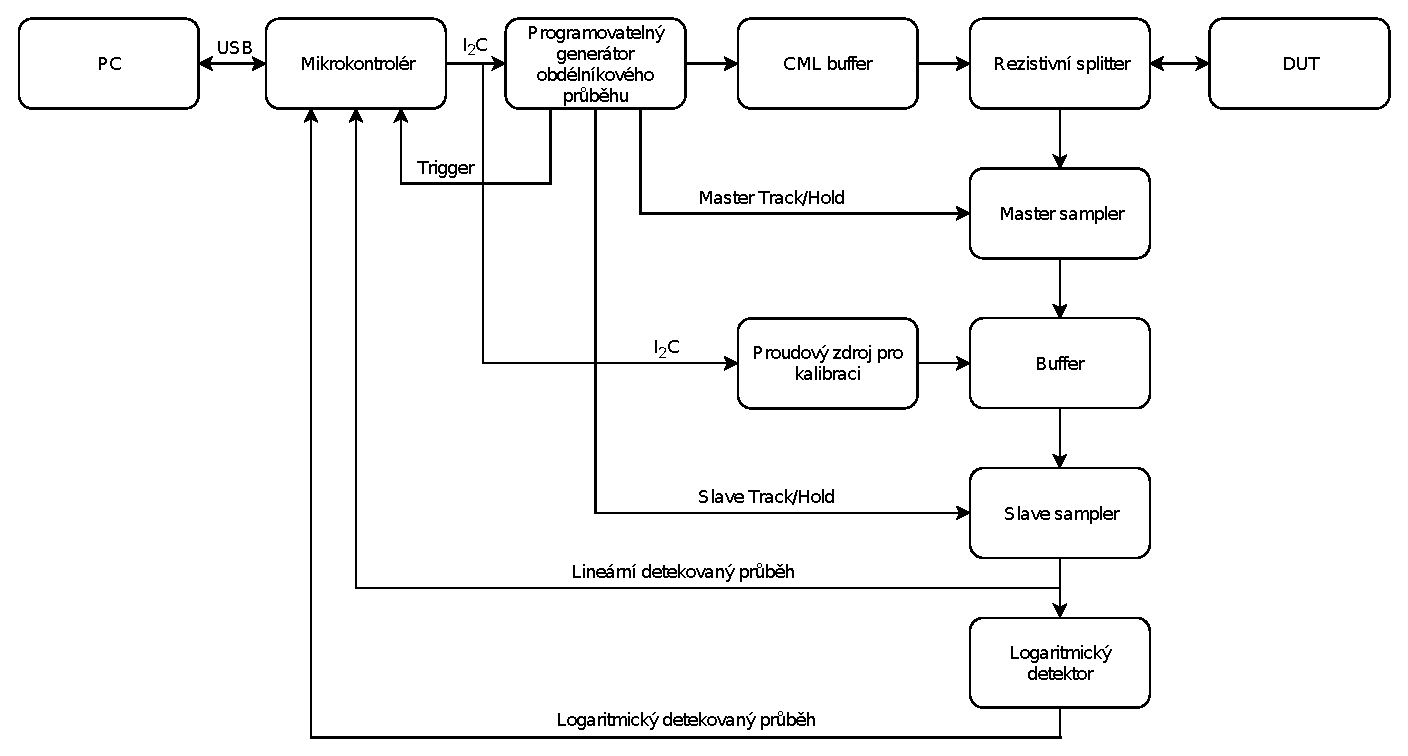
\includegraphics[width=\textwidth,height=12cm,keepaspectratio]{images/block_diagram.eps}\caption{Blokové zapojení reflektometru.} \label{block_diagram}
\end{figure}

Blokové zapojení reflektometru je znázorněno na obrázku \ref{block_diagram}. V dalších částech této kapitoly jsou jenotlivé bloky popsány do hloubky.

\section{Generování potřebných hodinových signálů}
Hlavním prvkem celého zapojení je vícekanálový digitální fázový závěs, který je postaven na obvodu Si5351C-B \cite{Si5351datasheet}. Tento obvod obsahuje krystalový oscilátor, na nějž jsou zavěšeny dva interní oscilátory \acrshort{VCO}. Vnitřní blokové schéma je možné vidět na obrázku \ref{si5351_internal_architecture_overview}.

\begin{figure}[htbp]
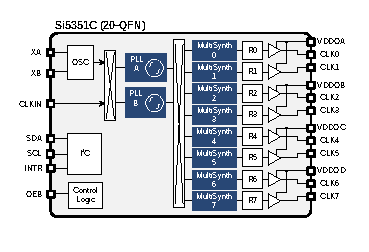
\includegraphics[width=\textwidth,height=12cm,keepaspectratio]{images/si5351_internal_architecture_overview.eps}\caption{Vnitřní blokové zapojení obvodu Si5351, převzato z \cite{Si5351datasheet}.} \label{si5351_internal_architecture_overview}
\end{figure}

Frekvenci těchto oscilátorů je možné nezávisle nastavit. Jejich frekvence $f_{VCO}$ může být neceločíselným násobkem frekvence krystalového oscilátoru $f_{XTAL}$.
\begin{equation}
f_{VCO}=f_{XTAL} \left(a+\dfrac{b}{c} \right)
\end{equation}
Koeficient $a$ může nabývat hodnot $\langle 15, 90 \rangle$. V neceločíselném režimu může koeficient $c$ nabývat hodnot $\langle 0, 1048575 \rangle$, koeficient $b$ pak $\langle 0, c \rangle$.
Je tedy možné nastavit frekvenci oscilátorů tak, že se liší o méně než 1 ppm. Při použití těchto dvou frekvencí jako časovacích signálů pro buzení a vzorkování je tedy možné odebírat až 1048576 vzorků. Dochází totiž k tomu, že s každou periodou se postupně hrany těchto obdélníkových signálů vůči sobě časově posunou o fixní časový krok. Tento krok je možné spočítat z nastavených frekvencí oscilátorů.

\begin{equation}
\begin{gathered}
f_{VCO1}=f_{XTAL} \left(a_1+\dfrac{b_1}{c_1} \right) \\
f_{VCO2}=f_{XTAL} \left(a_2+\dfrac{b_2}{c_2} \right)
\end{gathered}
\end{equation}

Za těmito oscilátory ještě následují děličky. Ty také umožňují neceločíselné dělení, které je ovšem nevýhodné, protože může zvyšovat fázové chvění výstupního signálu. Proto jsou použity pouze v celočíselném režimu. Děličky jsou použity kvůli omezenému vzorkovacímu kmitočtu použitého \acrshort{ADC}. Výsledkem jsou tedy dvě frekvence $f_{OUT1}$ a $f_{OUT2}$. Označíme-li společný dělicí poměr $d$ a za předpokladu, že $a_1=a_2=a$, $c_1=c_2=c$ a $b_2=0$:

\begin{equation}
\begin{gathered}
f_{OUT1}=\dfrac{f_{VCO1}}{d}=f_{XTAL} \left(\dfrac{a+\dfrac{b_1}{c} }{d}\right) \\
f_{OUT2}=\dfrac{f_{VCO2}}{d}=f_{XTAL} \left(\dfrac{a}{d}\right)
\end{gathered}
\end{equation}

Pak se během jedné periody oscilátory vůči sobě posunou o čas $T_{SHIFT}$:

\begin{equation}
\begin{gathered}
T_{SHIFT}=T_{OUT2}-T_{OUT1}=\dfrac{1}{f_{OUT2}} - \dfrac{1}{f_{OUT1}} \\
T_{SHIFT}=\dfrac{d}{f_{XTAL}} \left(\dfrac{1}{a} - \dfrac{1}{a+\dfrac{b_1}{c}}\right) = \dfrac{d}{f_{XTAL}} \left(\dfrac{1}{1+a\dfrac{c}{b_1}}\right)
\end{gathered}
\end{equation}

Pro minimalizaci fázového chvění je podle \cite{Si5351datasheet} a \cite{Si5351applicationnote} vhodné preferovat celočíselné násobení i dělení, je-li to možné. Dále může fázové chvění zmenšit i použití sudých násobitelů a dělitelů. V navrženém zapojení je tedy fázový závěs nastaven takto:

\begin{equation}
\begin{gathered}
f_{XTAL}= 25 \si{MHz} \\
a=24 \;\;\; b_1=1 \\
c=500000 \;\;\; d=128 \cdot 46 \\
f_{OUT1} \doteq 101902 \si{kHz} \doteq f_{OUT2} \\
T_{SHIFT} = \dfrac{46 \cdot 128}{25000000} \left(\dfrac{1}{1+24 \cdot \dfrac{500000}{1}}\right) \doteq 19.627 \si{ps}
\end{gathered}
\end{equation}

Podobný princip měření pomocí dvou oscilátorů o podobné frekvenci se již v literatuře objevil, avšak zatím nebyl implementován přímo pomocí fázového závěsu. V \cite{vernierreflectometer} byly použity dva nezávislé oscilátory. Toto řešení je sice jednodušší, avšak není možné zajistit, jak velký bude časový krok měření. Vzhledem ke skutečnosti, že oscilátory jsou závislé na teplotě a dalších vnějších vlivech, není možné zajistit ani dlouhodobou stabilitu. Při použití dvojitého fázového závěsu s neceločíselným násobitelem však je možné tuto dlouhodobou stabilitu zajistit. Krok měření je pak závislý pouze na frekvenci jediného krystalového oscilátoru. Při použití \acrshort{TCXO} může být tato stabilita velmi dobrá, na úrovni jednotek \si{ppm}.

Další podobný způsob časování vzorkování je použit v \cite{ddsfpgareflectometer}, kde je využito \acrshort{FPGA} jako \acrshort{DDS}. Výstup z této \acrshort{DDS} je filtrován dolní propustí a následně zaveden do komparátoru, římž je získáván obdélníkový řídicí signál. Řízení vzájemné polohy budicího pulzu a vzorkování je pak dosaženo nastavováním fáze sinusového signálu, který je generován \acrshort{DDS}. Tento systém umožňuje krok vzorkování v jednotkách pikosekund. Je tedy podobný vlastnostmi konstrukci popsané v této práci. Něvýhodou je však to, že autoři se příliš nezabývali generátorem impulzů, náběžná hrana použitého generátoru činí přibližně 2 \si{ns}. Důvod, proč tak autoři učinili, je možná omezení vyplývající ze zvoleného způsobu vzorkování pomocí komparátoru a digitálního integrátoru.

\begin{figure}[htbp]
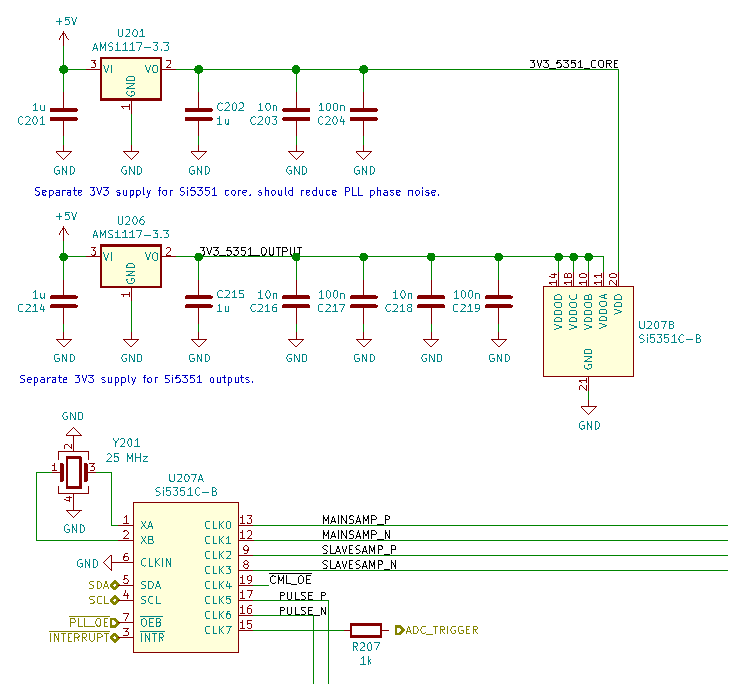
\includegraphics[width=\textwidth,height=12cm,keepaspectratio]{images/timing_section.eps}\caption{Zapojení hodinového generátoru Si5351.}\label{timing_section_schematic}
\end{figure}	

Zapojení hodinového generátoru s fázovým závěsem Si5351 je zobrazeno na \ref{timing_section_schematic}. Symbol obvodu je rozdělený na dvě části, U207A a U207B. Kromě samotného obvodu Si5351 je potřeba pouze referenční krystal a napájecí obvody. Napájení je rozděleno na dvě domény. První je jádro fázového závěsu, které napájí interní logické obvody a \acrshort{VCO}. Druhá napájí výstupní budiče. Toto rozdělení by mělo omezit fázový šum generovaných hodinových signálů způsobený rušením na napájení \acrshort{VCO} \cite{Si5351applicationnote}. Pro krystalový oscilátor není potřeba používat zatěžovací kondenzátory, jsou obsaženy uvnitř obvodu Si5351, je možné je nastavit v rozsahu \SIrange{4}{10}{\si{pF}}.

Výstupní budiče obvodu Si5351 jsou slučitelné jak s \acrshort{CMOS} obvody a jejich modernějšími variantami, tak i s obvody rodin \acrshort{TTL}, \acrshort{ECL}, \acrshort{CML}, \acrshort{LVDS} a podobnými. Budiče jsou proudové, proud je možné nastavit ve čtyřech krocích v rozsahu \SIrange{2}{8}{\si{mA}} \cite{Si5351datasheet}. Tohoto faktu je využito v zapojení, 4 výstupy jsou použity přímo pro proudové buzení vzorkovacích můstků, 2 výstupy pro buzení \acrshort{CML} bufferu, jeden výstup pro synchronizaci vzorkování použitého mikrokontroléru a jeden výstup pro řízení stavu \acrshort{CML} bufferu.

Dle katalogových údajů by tento fázový závěs měl typicky dosahovat mezivrcholového fázového šumu $70~\si{ps}$, maximálně  $155~\si{ps}$. Dle výrobce by mělo jít o parametry v \quotedblbase nejhorším možném případě v reálné aplikaci \ldots{} skutečné vlastnosti mohou být výrazně lepší\textquotedblleft{} \cite{Si5351datasheet}. Bohužel není uvedeno, jak se tento parametr mění v závislosti na nastavení násobicích a dělicích sekcí. Není uveden ani histogram šumu, jeho frekvenční spektrum, ani efektivní hodnota. Spektrum fázového šumu je možné najít v \cite{Si5351_phase_noise_measurement}, bohužel se nejedná o ověřený zdroj.

\section{Tvorba budicího pulzu}
Pro tvorbu budicích pulzů byl vybrán obvod SY54020, který je původně určen jako \acrshort{CML} buffer. Logické obvody \acrshort{CML} používají logické úrovně referencované vůči kladnému pólu napájení, výstupy i vstupy těchto obvodů jsou přizpůsobené impedanci $50~\Omega$. Podle katalogových údajů \cite{SY54020datasheet} by měla výstupní impedance ležet v rozsahu \SIrange{45}{55}{\si{$\Omega$}}. Hlavní důvod pro použití tohoto bufferu je vysoká rychlost, dle katalogových údajů by měla délka náběžných a sestupných hran spadat do rozsahu \SIrange{35}{100}{\si{ps}}, typicky $60~\si{ps}$. Tento údaj je udáván pro body, kde prochází náběžná hrana $20~\%$ a $80~\%$ mezi původním a konečným napětím. U obvodu Si5351 by podle katalogových údajů měl tento parametr být typicky $1~\si{ns}$, maximálně $1{,}5~\si{ns}$. Použitím obvodu SY54020 by tedy mělo být možné zkrátit náběžné hrany o \SIrange{90}{98}{\si{\%}} oproti přímému použití výstupu z obvodu Si5351 jako zdroje budicích pulzů.

Postatná výhoda obvodu SY54020 spočívá v oddělení napájecích úrovní vstupů a výstupů tohoto obvodu. V zapojení je vstupní část obvodu napájena $3{,}3~\si{V}$, výstupní část $1{,}65~\si{V}$, tedy přesně polovičním napájecím napětím. Tato napájecí hladina označená jako VCC, a zároveň jako GNDS, je použita jako virtuální analogová země. Všechny následující obvody jsou vztažené k této virtuální zemi.

Zapojení generátoru budicích impulzů je na obrázku \ref{pulse_generator_section_schematic}.

\begin{figure}[htbp]
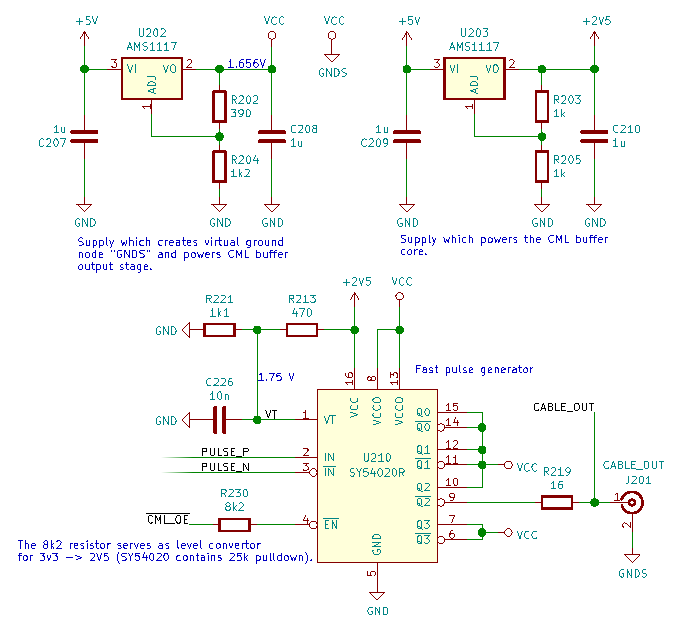
\includegraphics[width=\textwidth,height=12cm,keepaspectratio]{images/pulse_generator_section.eps}\caption{Zapojení generátoru budicích pulzů}\label{pulse_generator_section_schematic}
\end{figure}	

\section{Přizpůsobovací obvody a testovací port}
Generátor budicích impulzů z předchozího bodu je nezbytné připojit k měřicímu portu. K tomuto portu však musí být zároveň připojeny vzorkovací obvody. Proto jsou nezbytné přizpůsobovací obvody, které umožňují připojit k testovacímu portu obě tyto části při dodržení vstupní impedance. Jejich zapojení je uvedeno na obrázku \ref{match_section_schematic}.

\begin{figure}[htbp]
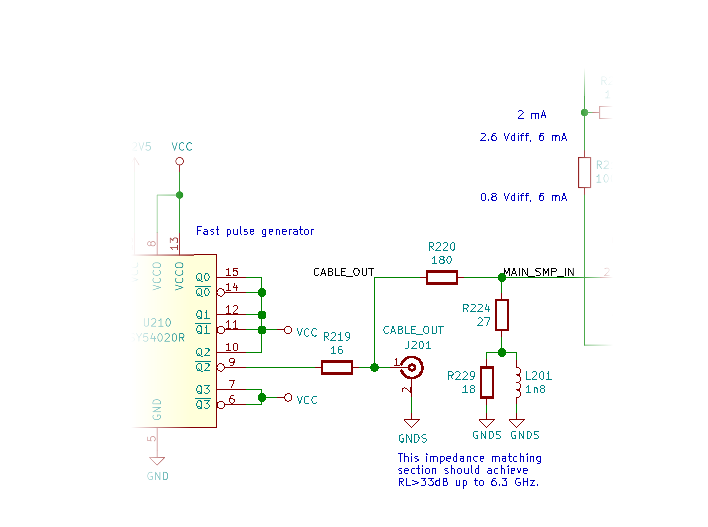
\includegraphics[width=\textwidth,height=12cm,keepaspectratio]{images/match_section.eps}\caption{Schéma přizpůsobovacích obvodů.}\label{match_section_schematic}
\end{figure}

Přizpůsobovací obvody jsou navrženy tak, aby bylo dosaženo co nejlepšího impedančního přizpůsobení na testovacím konektoru. Problematická je impedance vzorkovacího můstku, neboť na jeho výstupu je připojen vzorkovací kondenzátor, který způsobuje rezonanci pouzdra vzorkovacího můstku na frekvenci přibližně $1.7~\si{GHz}$. Vliv této rezonance na vstupní impedanci reflektometru je částečně potlačen tím, že 

\begin{figure}[htbp]
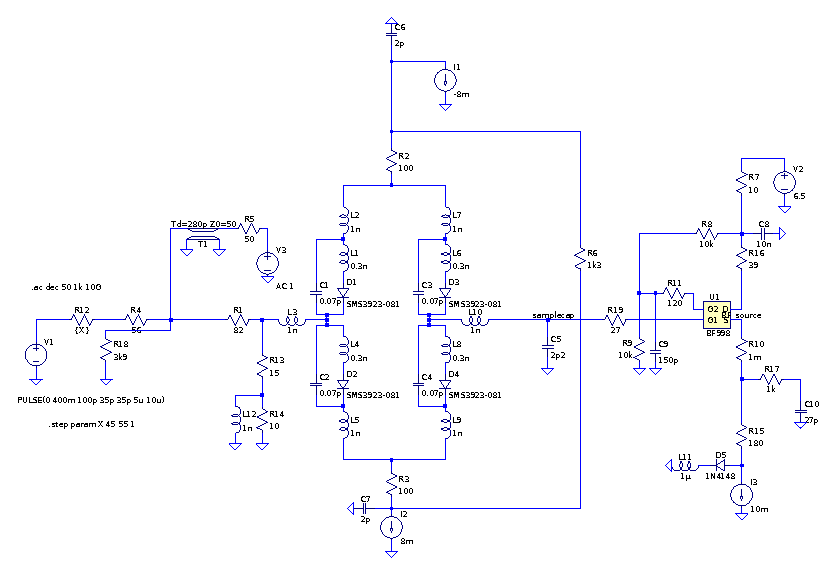
\includegraphics[width=\textwidth,height=12cm,keepaspectratio]{images/ltspice_schematic.eps}\caption{Schéma použité pro simulaci v programu LTSpice.}\label{ltspice_schematic}
\end{figure}

\begin{figure}[htbp]
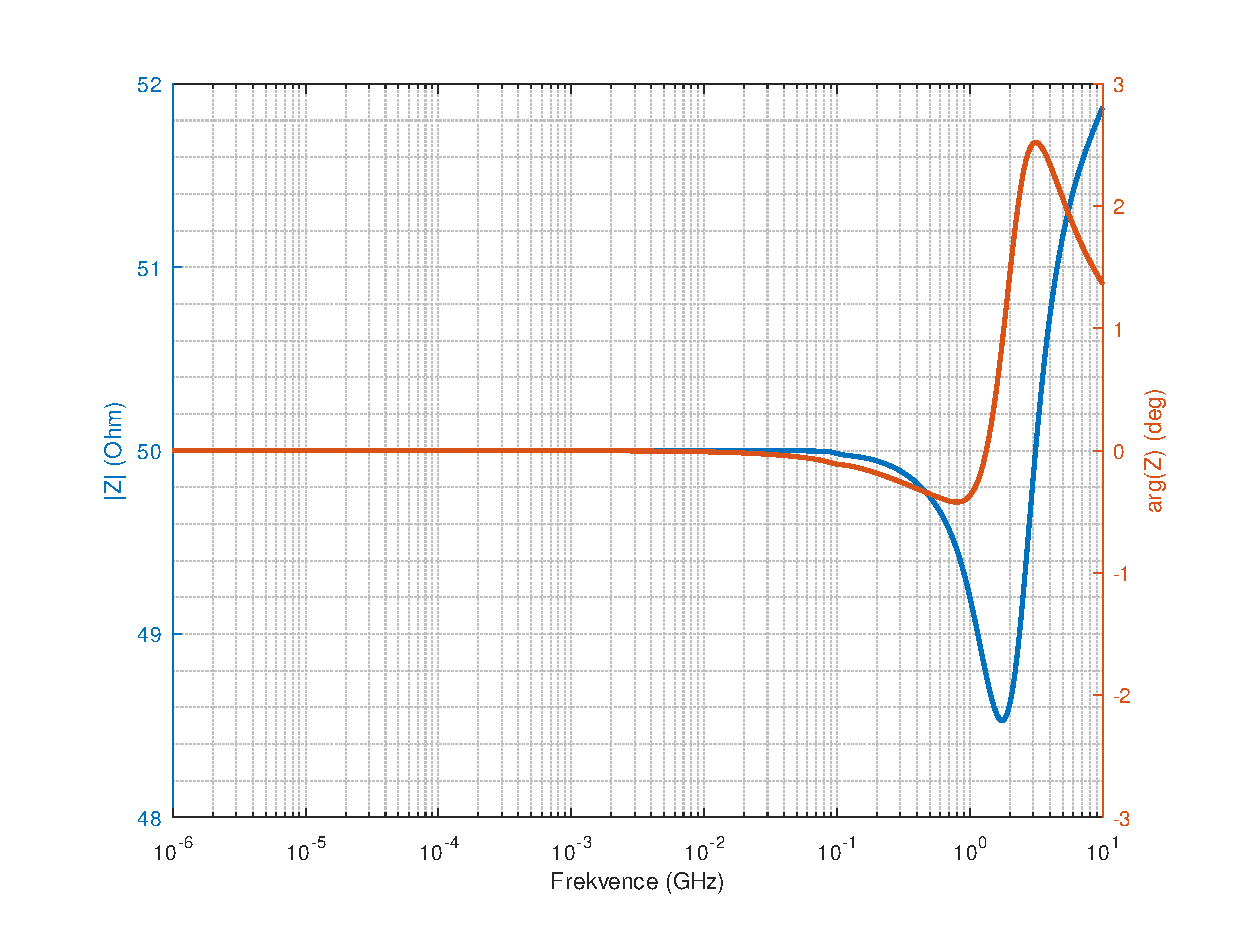
\includegraphics[width=\textwidth,height=12cm,keepaspectratio]{images/input_impedance.eps}\caption{Vstupní impedance reflektometru.}\label{input_impedance}
\end{figure}

\begin{figure}[htbp]
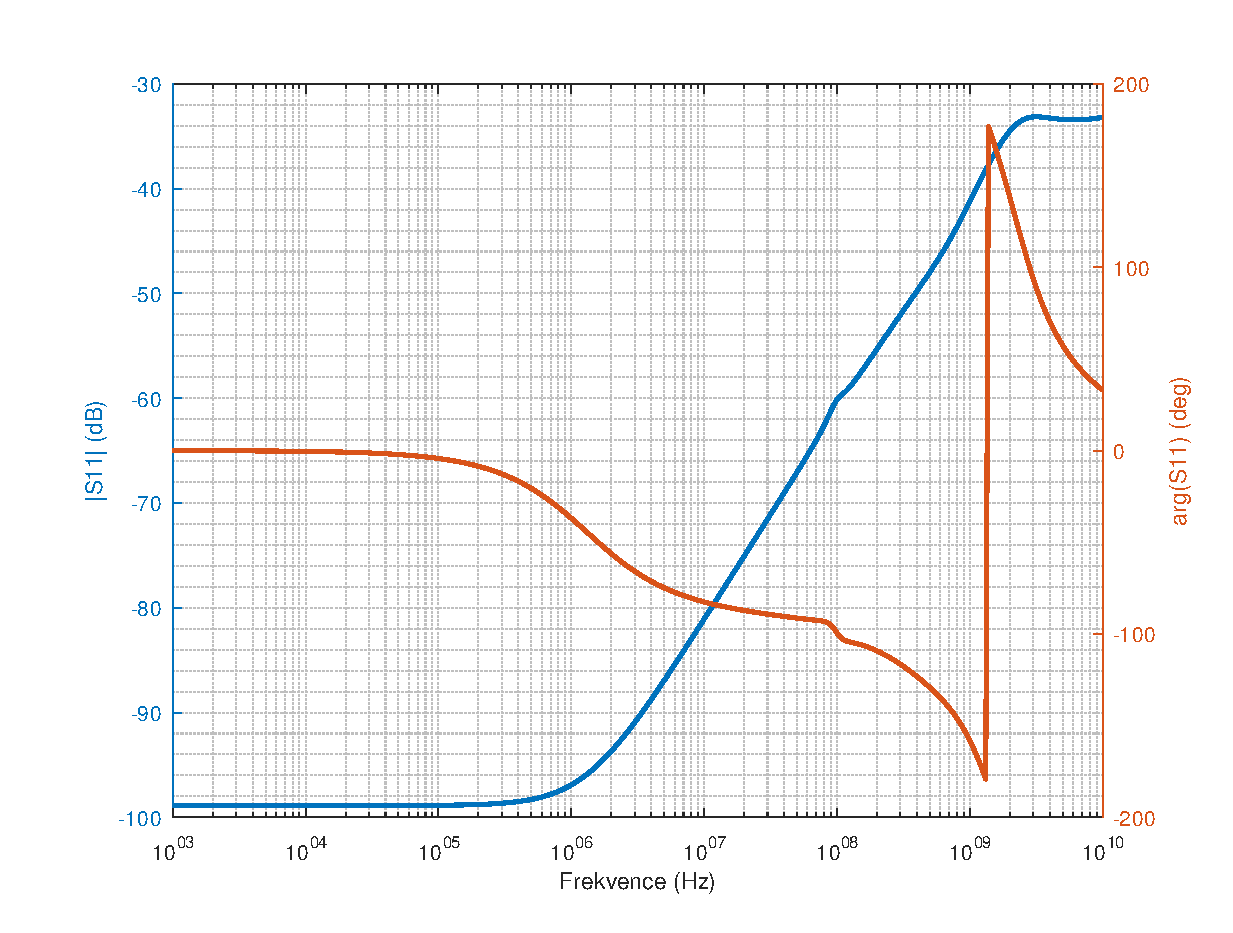
\includegraphics[width=\textwidth,height=12cm,keepaspectratio]{images/input_reflection.eps}\caption{Přizpůsobení vstupní impedance reflektometru.}\label{input_reflection}
\end{figure}


\section{Vzorkovací obvody}

\section{Oddělovací zesilovač}

\section{Sekundární vzorkování}

\section{Digitalizace měřeného průběhu}